\documentclass[11pt,a4paper]{article}

% --- Packages ---
\usepackage[utf8]{inputenc}
\usepackage[english]{babel}
\usepackage[T1]{fontenc}
\usepackage{lmodern}
\usepackage{geometry}
\geometry{left=1.8cm, right=1.8cm, top=1.8cm, bottom=1.8cm}
\usepackage{enumitem}
\usepackage{titlesec}
\usepackage{hyperref}
\usepackage{xcolor}
\usepackage{tabularx}
\usepackage{graphicx}

% --- Color Definitions ---
\definecolor{color0}{rgb}{0,0,0}         % Main text color (Black)
\definecolor{color1}{RGB}{0, 75, 135}    % Academic Blue
\definecolor{color2}{gray}{0.3}          % Secondary info color

% --- Section Styling ---
\titleformat{\section}
  {\Large\bfseries\color{color1}}
  {}{0em}{}
  [\titlerule]
\titlespacing{\section}{0pt}{14pt}{8pt}

% --- Hyperref Setup ---
\hypersetup{
    colorlinks=true,
    linkcolor=color1,
    urlcolor=color1,
    pdftitle={Davide Chirichella - Curriculum Vitae},
}

% --- Custom Entry Commands ---
\newcommand{\cvitem}[2]{
    \noindent
    \begin{tabularx}{\textwidth}{@{}p{3.8cm} X@{}}
        \textbf{#1} & #2
    \end{tabularx}
    \vspace{3pt}
}

\usepackage{etoolbox}
\newcommand{\cventry}[6]{
    \noindent
    \begin{tabularx}{\textwidth}{@{}p{3.8cm} X@{}}
        {\small\sffamily #1} & \textbf{#2} \\
        \ifstrempty{#3}{%
            \ifstrempty{#4}{%
                \ifstrempty{#5}{}{& \small #5 \\}%
            }{& #4\ifstrempty{#5}{}{\\ & \small #5} \\}%
        }{%
            & \textit{#3}\ifstrempty{#4}{}{, #4}\ifstrempty{#5}{}{\\ & \small #5} \\%
        }%
        & \small #6
    \end{tabularx}
    \vspace{10pt}
}

\begin{document}

\pagestyle{empty}

% --- Header ---
\noindent
\begin{minipage}[t]{0.80\textwidth}
    \raggedright
    {\Huge \textbf{Davide Chirichella}} \\
    \vspace{2mm}
    {\large \textcolor{color1}{Computer Engineering Master’s Student | Distributed Systems \& Junior DevOps Engineer}}
\end{minipage}
\begin{minipage}[t]{0.20\textwidth}
    \raggedleft
    \vspace{-4mm}
    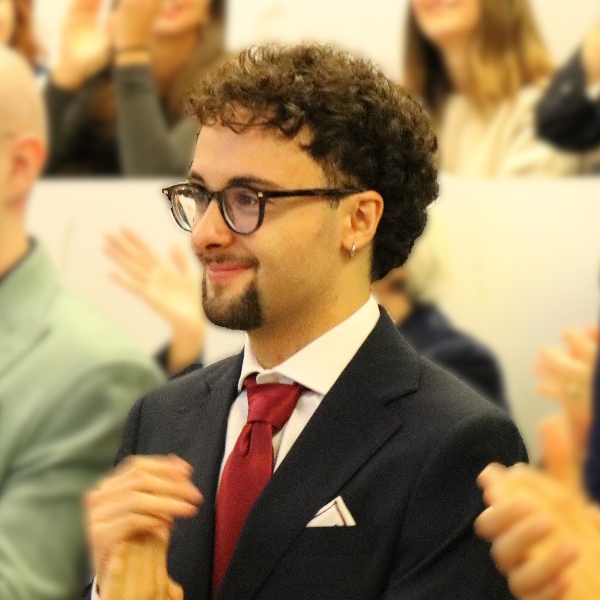
\includegraphics[width=2.1cm]{picture.png}
\end{minipage}

\vspace{4mm}

\section{Personal Information}
\cvitem{Full Name}{Davide Chirichella}
\cvitem{Date of Birth}{November 10th, 2003}
\cvitem{Citizenship}{Italian}
\cvitem{Current Location}{Bologna, Italy}
\cvitem{Email}{\href{mailto:davidechirichella10@gmail.com}{davidechirichella10@gmail.com} | \href{mailto:davide.chirichella@unibo.it}{davide.chirichella@unibo.it}}
\cvitem{LinkedIn}{\href{https://www.linkedin.com/in/davide-chirichella-88200b1ba/}{linkedin.com/in/davide-chirichella-88200b1ba}}
\cvitem{GitHub}{\href{https://github.com/chirichexe}{github.com/chirichexe}}

\section{Profile}
\noindent Junior engineer and Master’s student in \textbf{Computer Engineering} at the University of Bologna with hands-on experience in \textbf{distributed systems}, \textbf{cloud-native architectures}, and \textbf{DevOps practices}. Focused on designing and operating scalable microservices systems using Kubernetes and infrastructure-as-code. Experience spans backend development, CI/CD automation, and cloud-edge architectures for IoT environments.

\section{Education}
\cventry{2025 -- Present}{Master’s Degree in Computer Engineering}{Alma Mater Studiorum --- Università di Bologna}{Bologna}{Actual GPA: 29.5/30}{Focus on Distributed Systems, Parallel Computing, and Cloud-native architectures.}

\cventry{2022 -- 2025}{Bachelor’s Degree in Computer Engineering}{Alma Mater Studiorum --- Università di Bologna}{Bologna}{Grade: 107/110}{
\begin{itemize}[noitemsep, topsep=0pt, leftmargin=1em]
    \item \textbf{Thesis (Curricular Internship at DISI):} ``Performance Analysis and Monitoring in Cloud-Edge Environments for IoT''
    \item Developed a cloud-edge distributed system for orchestrating IoT devices using Kubernetes Operators, Crossplane, and Istio Service Mesh.
    \item Designed full observability stack with Prometheus, Grafana, and OpenTelemetry.
\end{itemize}}

\cventry{2017 -- 2022}{High School Diploma}{Liceo Scientifico Galileo Galilei}{Potenza}{}{Focus on Adobe Creative Cloud, Multimedia Content Production, and Graphic Design.}

\section{Experience}
\cventry{Feb 2026 -- Present}{Junior DevOps Engineer}{HoDiritto (Startup)}{Hybrid}{}{
\begin{itemize}[noitemsep, topsep=0pt, leftmargin=1em]
    \item Led the end-to-end system design and infrastructure architecture for an early-stage MVP.
    \item Managed service containerization and implemented API security best practices.
    \item Provisioned cloud infrastructure using Terraform and automated CI/CD pipelines.
    \item Configured the complete observability stack and handled the setup of DNS, servers, and corporate mail systems.
\end{itemize}}

\cventry{Feb 2026 -- Present}{Academic Tutor (System Administration)}{Alma Mater Studiorum --- Università di Bologna}{Bologna}{}{
\begin{itemize}[noitemsep, topsep=0pt, leftmargin=1em]
    \item Supported undergraduate course ``System Administration and Security''.
    \item Delivered hands-on guidance on Linux system administration, shell scripting, and security practices.
    \item Assisted students in debugging and system-level problem solving.
\end{itemize}}

\cventry{2023 -- 2026}{Software Engineer}{Project Quality Systems S.R.L.}{Remote}{}{
\begin{itemize}[noitemsep, topsep=0pt, leftmargin=1em]
    \item Developed and maintained a C\# desktop application for audit management.
    \item Designed and implemented full-stack features using React.js, Node.js, and MySQL.
    \item Contributed to the evolution of a corporate management platform.
    \item Collaborated in requirements analysis and feature design.
\end{itemize}}

\section{Projects}
\cventry{}{Cloud-Edge IoT Orchestration Platform (Internship project)}{}{}{}{
\begin{itemize}[noitemsep, topsep=0pt, leftmargin=1em]
    \item Designed a distributed architecture for managing low-power IoT devices across edge and cloud environments using Istio and Kubernetes.
    \item Implemented Kubernetes Custom Resources and controllers for device orchestration.
    \item Integrated Crossplane for dynamic infrastructure provisioning.
    \item Built observability pipeline using Prometheus, Grafana, and OpenTelemetry.
\end{itemize}}

\cventry{}{Open-source Contributions (GitHub)}{}{}{}{
\begin{itemize}[noitemsep, topsep=0pt, leftmargin=1em]
    \item Contributed to distributed systems and DevOps-related projects.
    \item Focus on Kubernetes tooling, automation, and cloud-native workflows.
\end{itemize}}

\section{Technical Skills}
\cvitem{Languages}{Go, C, Java, C\#, JavaScript (React.js, Node.js), Python, SQL, NoSQL databases, CUDA.}
\cvitem{Cloud \& DevOps}{Kubernetes, Docker, Terraform, Ansible, Vagrant, CI/CD pipelines, Istio, Crossplane.}
\cvitem{Observability}{Prometheus, Grafana, OpenTelemetry.}
\cvitem{Systems \& IoT}{Linux system administration, shell scripting, MQTT, Cybersecurity.}
\cvitem{Tools}{Git, Adobe Creative Suite (Photoshop, Illustrator, Premiere).}

\section{Languages}
\cvitem{Italian}{Native.}
\cvitem{English}{B2 - Cambridge English First (FCE).}

\vfill

\begin{minipage}[t]{0.5\textwidth}
    \raggedright
    \small Bologna, \today
\end{minipage}
\begin{minipage}[t]{0.5\textwidth}
    \raggedleft
    \small \textit{Davide Chirichella} \\[1.2cm]
    \rule{5cm}{0.4pt}
\end{minipage}

\vspace{1.5cm}
\noindent
\begin{minipage}{\textwidth}
    \centering
    \scriptsize
    Autorizzo il trattamento dei miei dati personali presenti nel curriculum vitae ai sensi del Decreto Legislativo 30 giugno 2003, n. 196 e dell’art. 13 del GDPR (Regolamento UE 2016/679) ai fini della ricerca e selezione del personale.
\end{minipage}

\end{document}
